%Lualatexで実行する

\documentclass{article}
\usepackage[most]{tcolorbox}
\usepackage{graphicx} % 画像の読み込みに必要
\usepackage{luatexja}
\usepackage{tikz}
\usetikzlibrary{shadings}

%南東に青い立体ボールを配置するコマンドを定義
\tcbset{
  myboxstyle/.style={
    enhanced,
    colback=white,
    colframe=black,
    sharp corners,
    overlay={
      \begin{scope}[shift={([xshift=-5mm,yshift=5mm]frame.south east)}]
        \shade[ball color=blue!70] (0,0) circle (5mm);
      \end{scope}
    }
  }
}
%%%

\begin{document}

%左上に小さなボックスを重ねる (\nodeで実現する!)
\begin{tcolorbox}[
  colback=cyan!20, % 水色の背景
  colframe=cyan!60!black,
  width=\linewidth,
  enhanced,
  overlay={
    % 緑の小さなボックス(左上に重ねる)+ 白枠 + 白文字
    \node[
      fill=green!60, % 背景色
      line width=3pt, % 枠線の太さ
      draw=white,               % 白い枠線
      text=white,               % 白文字
      minimum width=2cm,  % 横幅
      minimum height=0.5cm,  % 縦幅
      anchor=south west,  % 枠の南西を基準に合わせる
      font=\bfseries\small,     % 太字小さめ
      align=center              % 中央寄せ
    ] at ([xshift=-1mm, yshift=-2mm]frame.north west) {タイトル}; % atで重ねる位置を指定!shiftでずらせる!
  }
]
\centering
これは水色のボックスです。
\end{tcolorbox}

\bigskip



%画像をボックスに重ねる
\begin{tcolorbox}[
  colback=cyan!20,
  colframe=cyan!60!black,
  width=\linewidth, %0.6\linewidthとかにすると、横幅は小さくなる
  height=3cm,
  enhanced,
  overlay={
    % 左上に画像を重ねる例、innder sepはnodeの余白を調整
    \node[anchor=north west, inner sep=0pt] at ([xshift=1cm]frame.north west) {
      \includegraphics[width=1.5cm, height=1cm]{example-image}
    };
      
    % ボックスの中心から右へ1cmずらして画像を配置
    %\node[anchor=center, inner sep=0pt] at ([xshift=1cm]frame.center) {
      %\includegraphics[width=2cm]{example-image}
    %};
  }
]
\centering
これは水色のボックスです。\\
ボックスに画像を重ねた!
\end{tcolorbox}

\bigskip

% オプション引数 [2](第1引数:オプション、 第2引数:タイトル)
%1番目の引数だけがオプションとして、自動的に扱われる
% \newtcolorbox{環境名}[引数の個数N][1番目のオプション引数の初期値]{...}となっている。
\newtcolorbox{flexbox}[2][]{
  colback=yellow!10,
  colframe=blue!80!black,
  fonttitle=\bfseries,
  coltitle=green,
  title={#2},
  #1 % ← 追加オプションを引き継げる
}

\begin{flexbox}[colback=red!10]{注意}
背景色を上書きした例です。
\end{flexbox}

\bigskip



%環境を定義
% 引数あり(1つ)タイトルを受け取る
\newtcolorbox{mybox}{
enhanced,
drop fuzzy shadow,
colback=cyan!30,
colframe=cyan!30,
arc=5pt
}

\begin{mybox}
\centering
これはタイトル付きのボックスです。
\end{mybox}



\bigskip


%ボックス内にtikzで絵を描く。赤の立体ボールを書く
\begin{tcolorbox}[enhanced, colback=white]
  % tcolorbox内にTikZで球を描画
  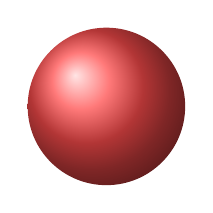
\begin{tikzpicture}
    \shade[ball color=red!70] (0,0) circle (1cm);
  \end{tikzpicture}

  立体的な球をtcolorbox内に描きました。
\end{tcolorbox}



\bigskip

%定義したコマンドを使用 (青の立体ボールを南東に配置)
\begin{tcolorbox}[myboxstyle]
ここは普通のテキストです。

右下(南東)に赤い立体的な球が見えます。
\end{tcolorbox}

\end{document}
